\documentclass[conference]{IEEEtran}
\IEEEoverridecommandlockouts
\usepackage{cite}
\usepackage{amsmath,amssymb,amsfonts}
\usepackage{algorithmic}
\usepackage{graphicx}
\usepackage{textcomp}
\usepackage{xcolor}
\usepackage{enumitem}
\def\BibTeX{{\rm B\kern-.05em{\sc i\kern-.025em b}\kern-.08em
    T\kern-.1667em\lower.7ex\hbox{E}\kern-.125emX}}

\begin{document}

\title{Conference Paper Title*\\
{\footnotesize \textsuperscript{*}Note: Sub-titles are not captured in Xplore and
should not be used}
\thanks{Identify applicable funding agency here. If none, delete this.}
}

\author{\IEEEauthorblockN{1\textsuperscript{st} Given Name Surname}
\IEEEauthorblockA{\textit{dept. name of organization (of Aff.)} \\
\textit{name of organization (of Aff.)}\\
City, Country \\
email address or ORCID}
\and
\IEEEauthorblockN{2\textsuperscript{nd} Given Name Surname}
\IEEEauthorblockA{\textit{dept. name of organization (of Aff.)} \\
\textit{name of organization (of Aff.)}\\
City, Country \\
email address or ORCID}
\and
\IEEEauthorblockN{3\textsuperscript{rd} Given Name Surname}
\IEEEauthorblockA{\textit{dept. name of organization (of Aff.)} \\
\textit{name of organization (of Aff.)}\\
City, Country \\
email address or ORCID}
\and
\IEEEauthorblockN{4\textsuperscript{th} Given Name Surname}
\IEEEauthorblockA{\textit{dept. name of organization (of Aff.)} \\
\textit{name of organization (of Aff.)}\\
City, Country \\
email address or ORCID}
\and
\IEEEauthorblockN{5\textsuperscript{th} Given Name Surname}
\IEEEauthorblockA{\textit{dept. name of organization (of Aff.)} \\
\textit{name of organization (of Aff.)}\\
City, Country \\
email address or ORCID}
\and
\IEEEauthorblockN{6\textsuperscript{th} Given Name Surname}
\IEEEauthorblockA{\textit{dept. name of organization (of Aff.)} \\
\textit{name of organization (of Aff.)}\\
City, Country \\
email address or ORCID}
}

\maketitle

\begin{abstract}
This document is a model and instructions for \LaTeX.
This and the IEEEtran.cls file define the components of your paper [title, text, heads, etc.]. *CRITICAL: Do Not Use Symbols, Special Characters, Footnotes, 
or Math in Paper Title or Abstract.
\end{abstract}

\begin{IEEEkeywords}
component, formatting, style, styling, insert
\end{IEEEkeywords}

\section{Introduction}
This document is a model and instructions for \LaTeX.
Please observe the conference page limits. 

\section{Ease of Use}

\subsection{Maintaining the Integrity of the Specifications}

The IEEEtran class file is used to format your paper and style the text. All margins, 
column widths, line spaces, and text fonts are prescribed; please do not 
alter them. You may note peculiarities. For example, the head margin
measures proportionately more than is customary. This measurement 
and others are deliberate, using specifications that anticipate your paper 
as one part of the entire proceedings, and not as an independent document. 
Please do not revise any of the current designations.

\section{AI Toolkits and Potential Applications for Mobile Networks}
\textcolor{blue}{The integration of Artificial Intelligence (AI) into the Radio Access Network (RAN) represents a paradigm shift from traditional, human-driven optimization to intelligent, autonomous network control. However, bridging the gap between advanced AI models and the real-time, high-stakes environment of a mobile network requires a new class of foundational software. AI toolkits for the RAN are specialized frameworks designed to address this challenge, providing the essential infrastructure to develop, deploy, and manage AI-driven applications within the complex cellular architecture.}

\textcolor{blue}{The primary goal of these toolkits is to streamline the entire AI workflow by addressing three critical pillars:}

\begin{enumerate}
\renewcommand\labelitemi{\textcolor{blue}{\textbullet}}
\renewcommand\labelenumi{\textcolor{blue}{\theenumi.}}
\color{blue}
\item GPU-Acceleration: The RAN operates under extremely strict latency constraints. These toolkits provide optimized libraries that leverage the parallel processing power of Graphics Processing Units (GPUs) to ensure that sophisticated AI algorithms can execute within the real-time budget of the RAN.

\item Data Processing and Management: A modern RAN is a prolific source of data. AI toolkits offer robust data pipelines to ingest, aggregate, and pre-process this high-velocity data, transforming it into a clean, model-ready format.

\item AI Lifecycle Management (MLOps): The operational challenge lies in managing thousands of models distributed across a live network. These toolkits incorporate MLOps principles tailored for telecommunications, automating the end-to-end lifecycle of AI models to ensure they remain robust, secure, and effective over time.

\end{enumerate}

\textcolor{blue}{In essence, AI toolkits serve as the critical enabling layer, abstracting away the underlying hardware and data complexity to empower developers and operators to build and operate a truly intelligent RAN.}

\subsection{AI toolkits}\label{AA}

\textcolor{blue}{NVIDIA provides several advanced AI toolkits that accelerate the design, testing, and operation of current and future wireless communication systems, including 5G and 6G.}

\textcolor{blue}{
\subsubsection{RAN-Specific Platforms \& SDKs}
\textcolor{blue}{While the concept of an AI toolkit is broad, several industry players offer specific platforms and SDKs. An exemplary platform is the NVIDIA Aerial SDK, a complete software stack for building high-performance, GPU-accelerated, cloud-native 5G and 6G virtualized RANs (vRANs). Its architecture is centered on two core libraries:}}


\begin{itemize}

\item \textcolor{blue}{cuBB (CUDA Baseband): Regarded as the ``heart of Aerial,'' it acts as the signal processing engine by implementing the entire L1-L2 stack (cuPHY and cuMAC) on the GPU, ensuring high throughput by keeping all processing within high-performance GPU memory.}

\item \textcolor{blue}{cuVNF (CUDA Virtual Network Functions): This SDK serves as the I/O engine, providing optimised input/output directly to GPU memory from GPUDirect-capable Network Interface Cards (NICs).}
\end{itemize}

\begin{figure}[htbp]
\centerline{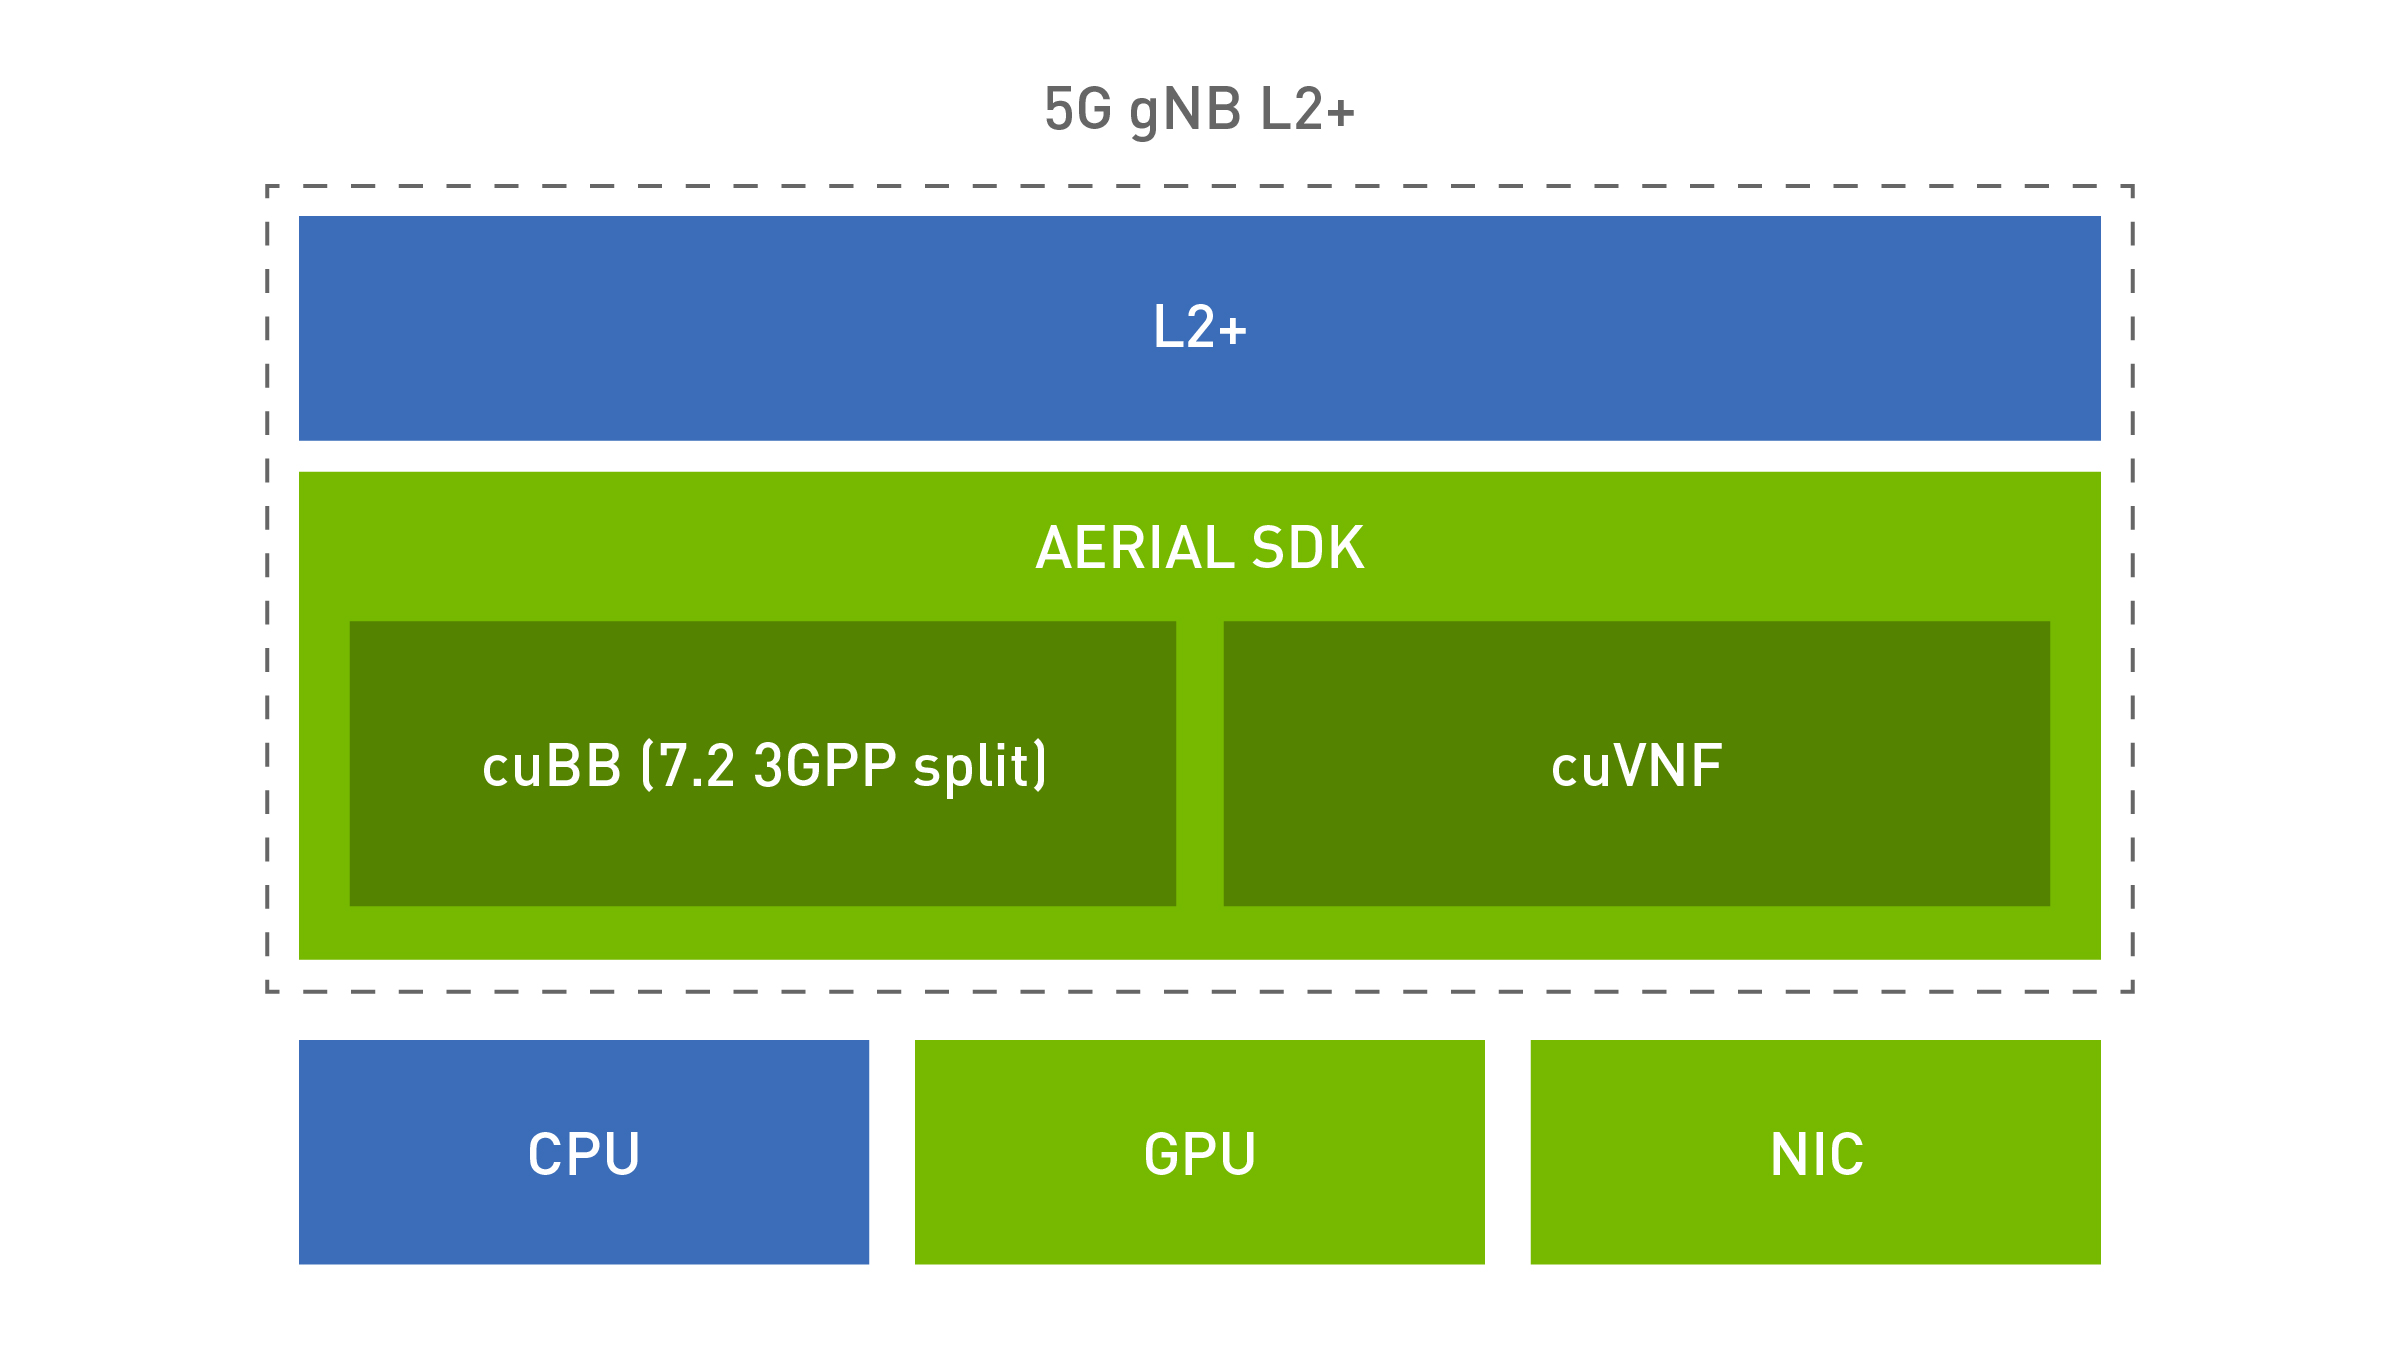
\includegraphics[width=0.9\columnwidth]{images/nvidia_aerial_sdk.jpg}}
\caption{NVIDIA Aerial SDK platform for GPU-accelerated, cloud-native vRANs.}
\label{fig:nvidia_aerial_sdk}
\end{figure}

\textcolor{blue}{The broader market of established vendors is also integrating AI. Qualcomm focuses on powerful hardware like the X100 Accelerator Card for inline acceleration. Ericsson embeds AI deeply into its solutions via its Intelligent RAN Automation portfolio. Nokia offers both a commercial RAN Intelligent Controller (RIC) and integrates AI into its AirScale baseband portfolio.}

\textcolor{blue}{\subsubsection{The O-RAN Architectural Framework}
The O-RAN Alliance defines a disaggregated and intelligent architecture for the RAN, centered on the RAN Intelligent Controller (RIC). The RIC functions as the network's "operating system," enabling AI-driven control via a modular, app-based model. It is split into the Non-Real-Time RIC (for network-wide policies via rApps) and the Near-Real-Time RIC (for low-latency control via xApps).}

\textcolor{blue}{\subsubsection{Simulation and Data Generation Toolkits}
The development of robust AI models is critically dependent on large, high-quality datasets. Simulation toolkits fill this gap.}

\begin{itemize}
\item \textcolor{blue}{NVIDIA Sionna: An open-source, Python-based library for link-level simulation. It is designed for communications research and enables the rapid prototyping of AI/ML systems for the physical layer. It includes modules for ray tracing (Sionna RT), link-level simulation (Sionna PHY), and system-level simulation (Sionna SYS). A key component is the Sionna Research Kit (SRK), which enables the deployment of trained models into a real software-defined 5G network on the NVIDIA Jetson AGX Orin platform.}

\item \textcolor{blue}{NVIDIA Aerial Omniverse Digital Twin (AODT): A next-generation, system-level simulation platform for R\&D on 5G/6G systems. AODT applies ray-traced channels to the NVIDIA Aerial RAN platform, simulating the system-level performance of an actual network deployment without abstractions. It is a unique tool to benchmark performance and explore ML algorithms under real-world conditions.}
\end{itemize}

\begin{figure}[htbp]
\centerline{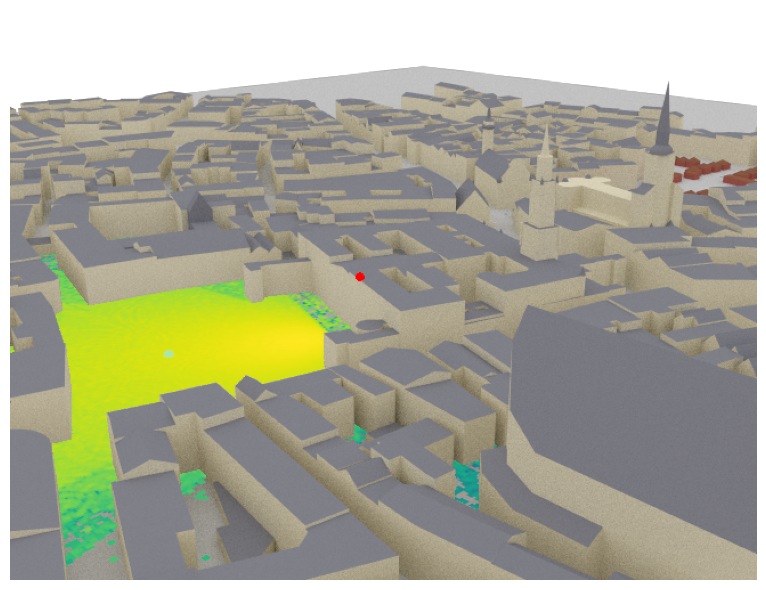
\includegraphics[width=0.9\columnwidth]{images/nvidia_sionna_simulation.png}}
\caption{NVIDIA Sionna simulation toolkit for AI-native air interface research.}
\label{fig:nvidia_sionna_simulation}
\end{figure}


\textcolor{blue}{\subsubsection{General Purpose \& Emerging Toolkits}
A new frontier in network automation is the application of Large Language Models (LLMs) and Generative AI (GenAI). Toolkits involving models like Gemini, coupled with the Retrieval-Augmented Generation (RAG) technique, are being explored for complex network operations like automated root cause analysis, configuration script generation, and interactive troubleshooting.}

\subsection{Technical feasibility}
\textcolor{blue}{The introduction of the AI toolkits described raises critical questions about their practical implementation and technological readiness. This section assesses the technical feasibility, focusing on their performance, data dependency, maturity, and operational robustness.}

\textcolor{blue}{\subsubsection{Model Performance and Algorithmic Efficiency}
The feasibility of toolkits like the NVIDIA Aerial SDK and the O-RAN RIC hinges on their ability to execute AI algorithms within the RAN’s stringent latency budgets. For platforms such as Aerial, which move L1 processing to GPUs, the key feasibility question is whether this software-defined approach can consistently match or exceed the performance of traditional hardware while simultaneously running AI models for real-time tasks like beam management. Similarly, for the O-RAN framework, the performance of an xApp is constrained by the processing capacity of the Near-RT RIC platform it runs on and the latency of the E2 interface, making algorithmic efficiency a non-negotiable requirement for any viable application.}

\textcolor{blue}{\subsubsection{Data Availability and Accessibility}
The AI toolkits discussed are fundamentally dependent on data. For toolkits aimed at the physical layer, like NVIDIA Sionna, feasibility is enhanced by its ability to synthetically generate high-fidelity training data. For emerging GenAI toolkits, feasibility depends on creating robust RAG pipelines that can interpret diverse operator data sources.}

\textcolor{blue}{\subsubsection{Technology Maturity and Integration}
While individual technologies are maturing, their integration poses a significant technical challenge. The NVIDIA Aerial SDK is a mature product, but its feasibility depends on seamless integration into a multi-vendor vRAN ecosystem. The O-RAN framework itself represents a major integration challenge focused on interoperability.}

\textcolor{blue}{\subsubsection{Security, Reliability, and Scalability}
For these toolkits to be technically feasible, they must meet telco-grade requirements. The reliability of a software-defined stack like NVIDIA Aerial must be proven to match the "five-nines" (99.999\%) availability of traditional hardware. The scalability of managing thousands of unique xApp instances across a national network poses a significant MLOps challenge.}

\subsection{Potential applications in mobile networks}
\textcolor{blue}{The surveyed toolkits facilitate a range of high-impact use cases for building intelligent mobile networks:}

\begin{itemize}
\item \textcolor{blue}{AI-Native Air Interface: The NVIDIA Aerial SDK enables the development of highly programmable and scalable 5G vRANs where AI/ML frameworks can be seamlessly integrated for real-time signal processing.}

\item \textcolor{blue}{System-Level R\&D and Optimization: The NVIDIA AODT allows researchers to benchmark system performance, explore ML-based algorithms, and optimize network planning using physically accurate simulations without abstractions.}

\item \textcolor{blue}{Rapid Prototyping and Deployment: NVIDIA Sionna accelerates research into 6G by enabling fast, GPU-accelerated modeling of communication systems, while its Sionna Research Kit (SRK) bridges the gap from research to reality by enabling deployment into a real software-defined 5G network.}
\end{itemize}

\subsection{Deployment constraints in mobile networks}

\textcolor{blue}{The practical deployment of the surveyed AI toolkits is constrained by a series of specific hardware and software requirements that must be met for successful implementation and operation. These are not theoretical challenges but concrete prerequisites essential for the toolkits to function correctly within a mobile network. Successful deployment hinges on the availability of powerful and specific hardware, including particular NVIDIA GPUs, qualified server systems like the Dell R750, and substantial system memory. Furthermore, the software environment must be precisely configured, mandating specific versions of operating systems, drivers, and libraries like CUDA and TensorFlow, often necessitating the use of containerized environments.}

\textcolor{blue}{\subsubsection{NVIDIA Aerial Omniverse Digital Twin (AODT)}}

\textcolor{blue}{\textbf{Hardware:} Requires specific NVIDIA GPUs with substantial vRAM (e.g., RTX 6000 Ada with 12GB+ for frontend; A100/H100 with 48GB+ for backend). Qualified systems include Dell R750 servers with Intel Xeon Gold CPUs and 512GB DDR4 Memory.}

\textcolor{blue}{\textbf{Software:} The backend requires Ubuntu 22.04. The frontend supports Ubuntu 22.04 and Windows 11. Specific NVIDIA driver versions are required (e.g., 560.35.05 for Linux backend).}

\textcolor{blue}{\subsubsection{NVIDIA Aerial SDK}}

\textcolor{blue}{\textbf{Hardware:} Runs on NVIDIA-certified EGX servers. Qualified platforms use GPUs like the NVIDIA A100x, DPUs like the Mellanox CX6-DX, and CPUs such as the Intel Xeon Gold 6336Y. Memory ranges from 96GB to 512GB of DDR4 RAM.}

\textcolor{blue}{\textbf{Software:} Requires a specific stack, including Ubuntu 20.04 with a low-latency kernel, CUDA 11.7 Toolkit, and Kubernetes version 1.23.}

\textcolor{blue}{\subsubsection{NVIDIA Sionna}}

\textcolor{blue}{\textbf{Hardware:} While GPU-accelerated for performance, Sionna can also run on a CPU. The Sionna Research Kit (SRK) component is specifically designed for the NVIDIA Jetson AGX Orin platform.}

\textcolor{blue}{\textbf{Software:} Requires Python 3.8-3.12 and TensorFlow 2.14-2.19. Ubuntu 24.04 is the recommended operating system. A Docker container or Python virtual environment is highly recommended.}

{\BibTeX} does not work by magic. It doesn't get the bibliographic
data from thin air but from .bib files. If you use {\BibTeX} to produce a
bibliography you must send the .bib files. 

{\LaTeX} can't read your mind. If you assign the same label to a
subsubsection and a table, you might find that Table I has been cross
referenced as Table IV-B3. 

{\LaTeX} does not have precognitive abilities. If you put a
\verb|\label| command before the command that updates the counter it's
supposed to be using, the label will pick up the last counter to be
cross referenced instead. In particular, a \verb|\label| command
should not go before the caption of a figure or a table.

Do not use \verb|\nonumber| inside the \verb|{array}| environment. It
will not stop equation numbers inside \verb|{array}| (there won't be
any anyway) and it might stop a wanted equation number in the
surrounding equation.

\subsection{Some Common Mistakes}\label{SCM}
\begin{itemize}
\item The word ``data'' is plural, not singular.
\item The subscript for the permeability of vacuum $\mu_{0}$, and other common scientific constants, is zero with subscript formatting, not a lowercase letter ``o''.
\item In American English, commas, semicolons, periods, question and exclamation marks are located within quotation marks only when a complete thought or name is cited, such as a title or full quotation. When quotation marks are used, instead of a bold or italic typeface, to highlight a word or phrase, punctuation should appear outside of the quotation marks. A parenthetical phrase or statement at the end of a sentence is punctuated outside of the closing parenthesis (like this). (A parenthetical sentence is punctuated within the parentheses.)
\item A graph within a graph is an ``inset'', not an ``insert''. The word alternatively is preferred to the word ``alternately'' (unless you really mean something that alternates).
\item Do not use the word ``essentially'' to mean ``approximately'' or ``effectively''.
\item In your paper title, if the words ``that uses'' can accurately replace the word ``using'', capitalize the ``u''; if not, keep using lower-cased.
\item Be aware of the different meanings of the homophones ``affect'' and ``effect'', ``complement'' and ``compliment'', ``discreet'' and ``discrete'', ``principal'' and ``principle''.
\item Do not confuse ``imply'' and ``infer''.
\item The prefix ``non'' is not a word; it should be joined to the word it modifies, usually without a hyphen.
\item There is no period after the ``et'' in the Latin abbreviation ``et al.''.
\item The abbreviation ``i.e.'' means ``that is'', and the abbreviation ``e.g.'' means ``for example''.
\end{itemize}

\subsection{Authors and Affiliations}
\textbf{The class file is designed for, but not limited to, six authors.} A 
minimum of one author is required for all conference articles. Author names 
should be listed starting from left to right and then moving down to the 
next line. This is the author sequence that will be used in future citations 
and by indexing services. Names should not be listed in columns nor group by 
affiliation. Please keep your affiliations as succinct as possible (for 
example, do not differentiate among departments of the same organization).

\subsection{Identify the Headings}
Headings, or heads, are organizational devices that guide the reader through 
your paper. There are two types: component heads and text heads.

Component heads identify the different components of your paper and are not 
topically subordinate to each other. Examples include Acknowledgments and 
References and, for these, the correct style to use is ``Heading 5''. Use 
``figure caption'' for your Figure captions, and ``table head'' for your 
table title. Run-in heads, such as ``Abstract'', will require you to apply a 
style (in this case, italic) in addition to the style provided by the drop 
down menu to differentiate the head from the text.

Text heads organize the topics on a relational, hierarchical basis. For 
example, the paper title is the primary text head because all subsequent 
material relates and elaborates on this one topic. If there are two or more 
sub-topics, the next level head (uppercase Roman numerals) should be used 
and, conversely, if there are not at least two sub-topics, then no subheads 
should be introduced.

\subsection{Figures and Tables}
\paragraph{Positioning Figures and Tables} Place figures and tables at the top and 
bottom of columns. Avoid placing them in the middle of columns. Large 
figures and tables may span across both columns. Figure captions should be 
below the figures; table heads should appear above the tables. Insert 
figures and tables after they are cited in the text. Use the abbreviation 
``Fig.~\ref{fig:nvidia_aerial_sdk}'' or ``Fig.~\ref{fig:nvidia_sionna_simulation}'', even at the beginning of a sentence.

\begin{table}[htbp]
\caption{Table Type Styles}
\begin{center}
\begin{tabular}{|c|c|c|c|}
\hline
\textbf{Table}&\multicolumn{3}{|c|}{\textbf{Table Column Head}} \\
\cline{2-4} 
\textbf{Head} & \textbf{\textit{Table column subhead}}& \textbf{\textit{Subhead}}& \textbf{\textit{Subhead}} \\
\hline
copy& More table copy$^{\mathrm{a}}$& &  \\
\hline
\multicolumn{4}{l}{$^{\mathrm{a}}$Sample of a Table footnote.}
\end{tabular}
\label{tab1}
\end{center}
\end{table}

\begin{figure}[htbp]
\centerline{
\includegraphics{fig1.png}}
\caption{Sample figure referenced in the text.}
\label{fig}
\end{figure}

\section{Conclusion}
The integration of artificial intelligence is a critical component of the roadmap to 6G wireless networks \cite{letaief_roadmap_2019}. This has spurred the development of advanced toolkits from major industry players. For example, established vendors like Ericsson are offering platforms for intelligent RAN automation \cite{ericsson_iran_2025}.

At a more granular level, NVIDIA provides a suite of tools for building GPU-accelerated RAN. This includes detailed software components for the baseband and physical layers, such as the Aerial cuBB and cuPHY \cite{nvidia_cubb_quickstart_2025, nvidia_cuphy_overview_2025}. Furthermore, to facilitate the research and training of AI models for these new systems, simulation libraries like NVIDIA Sionna have become essential \cite{nvidia_sionna_2025}.

{\color{blue}
\bibliographystyle{IEEEtran}
\bibliography{references}
}
\end{document}
